\chapter*{基础知识补充}
\addcontentsline{toc}{chapter}{基础知识补充}
\markboth{基础知识补充}{基础知识补充}

\section{三角函数}
\subsection{三角函数图像及性质}
\textbf{正切函数与余切函数}

正切函数$y=\tan x$(见图\ref{tan}),余切函数$y=\cot x$(见图\ref{cot})
\begin{figure}[H]
\centering
\begin{minipage}{0.4\linewidth}
    \centerline{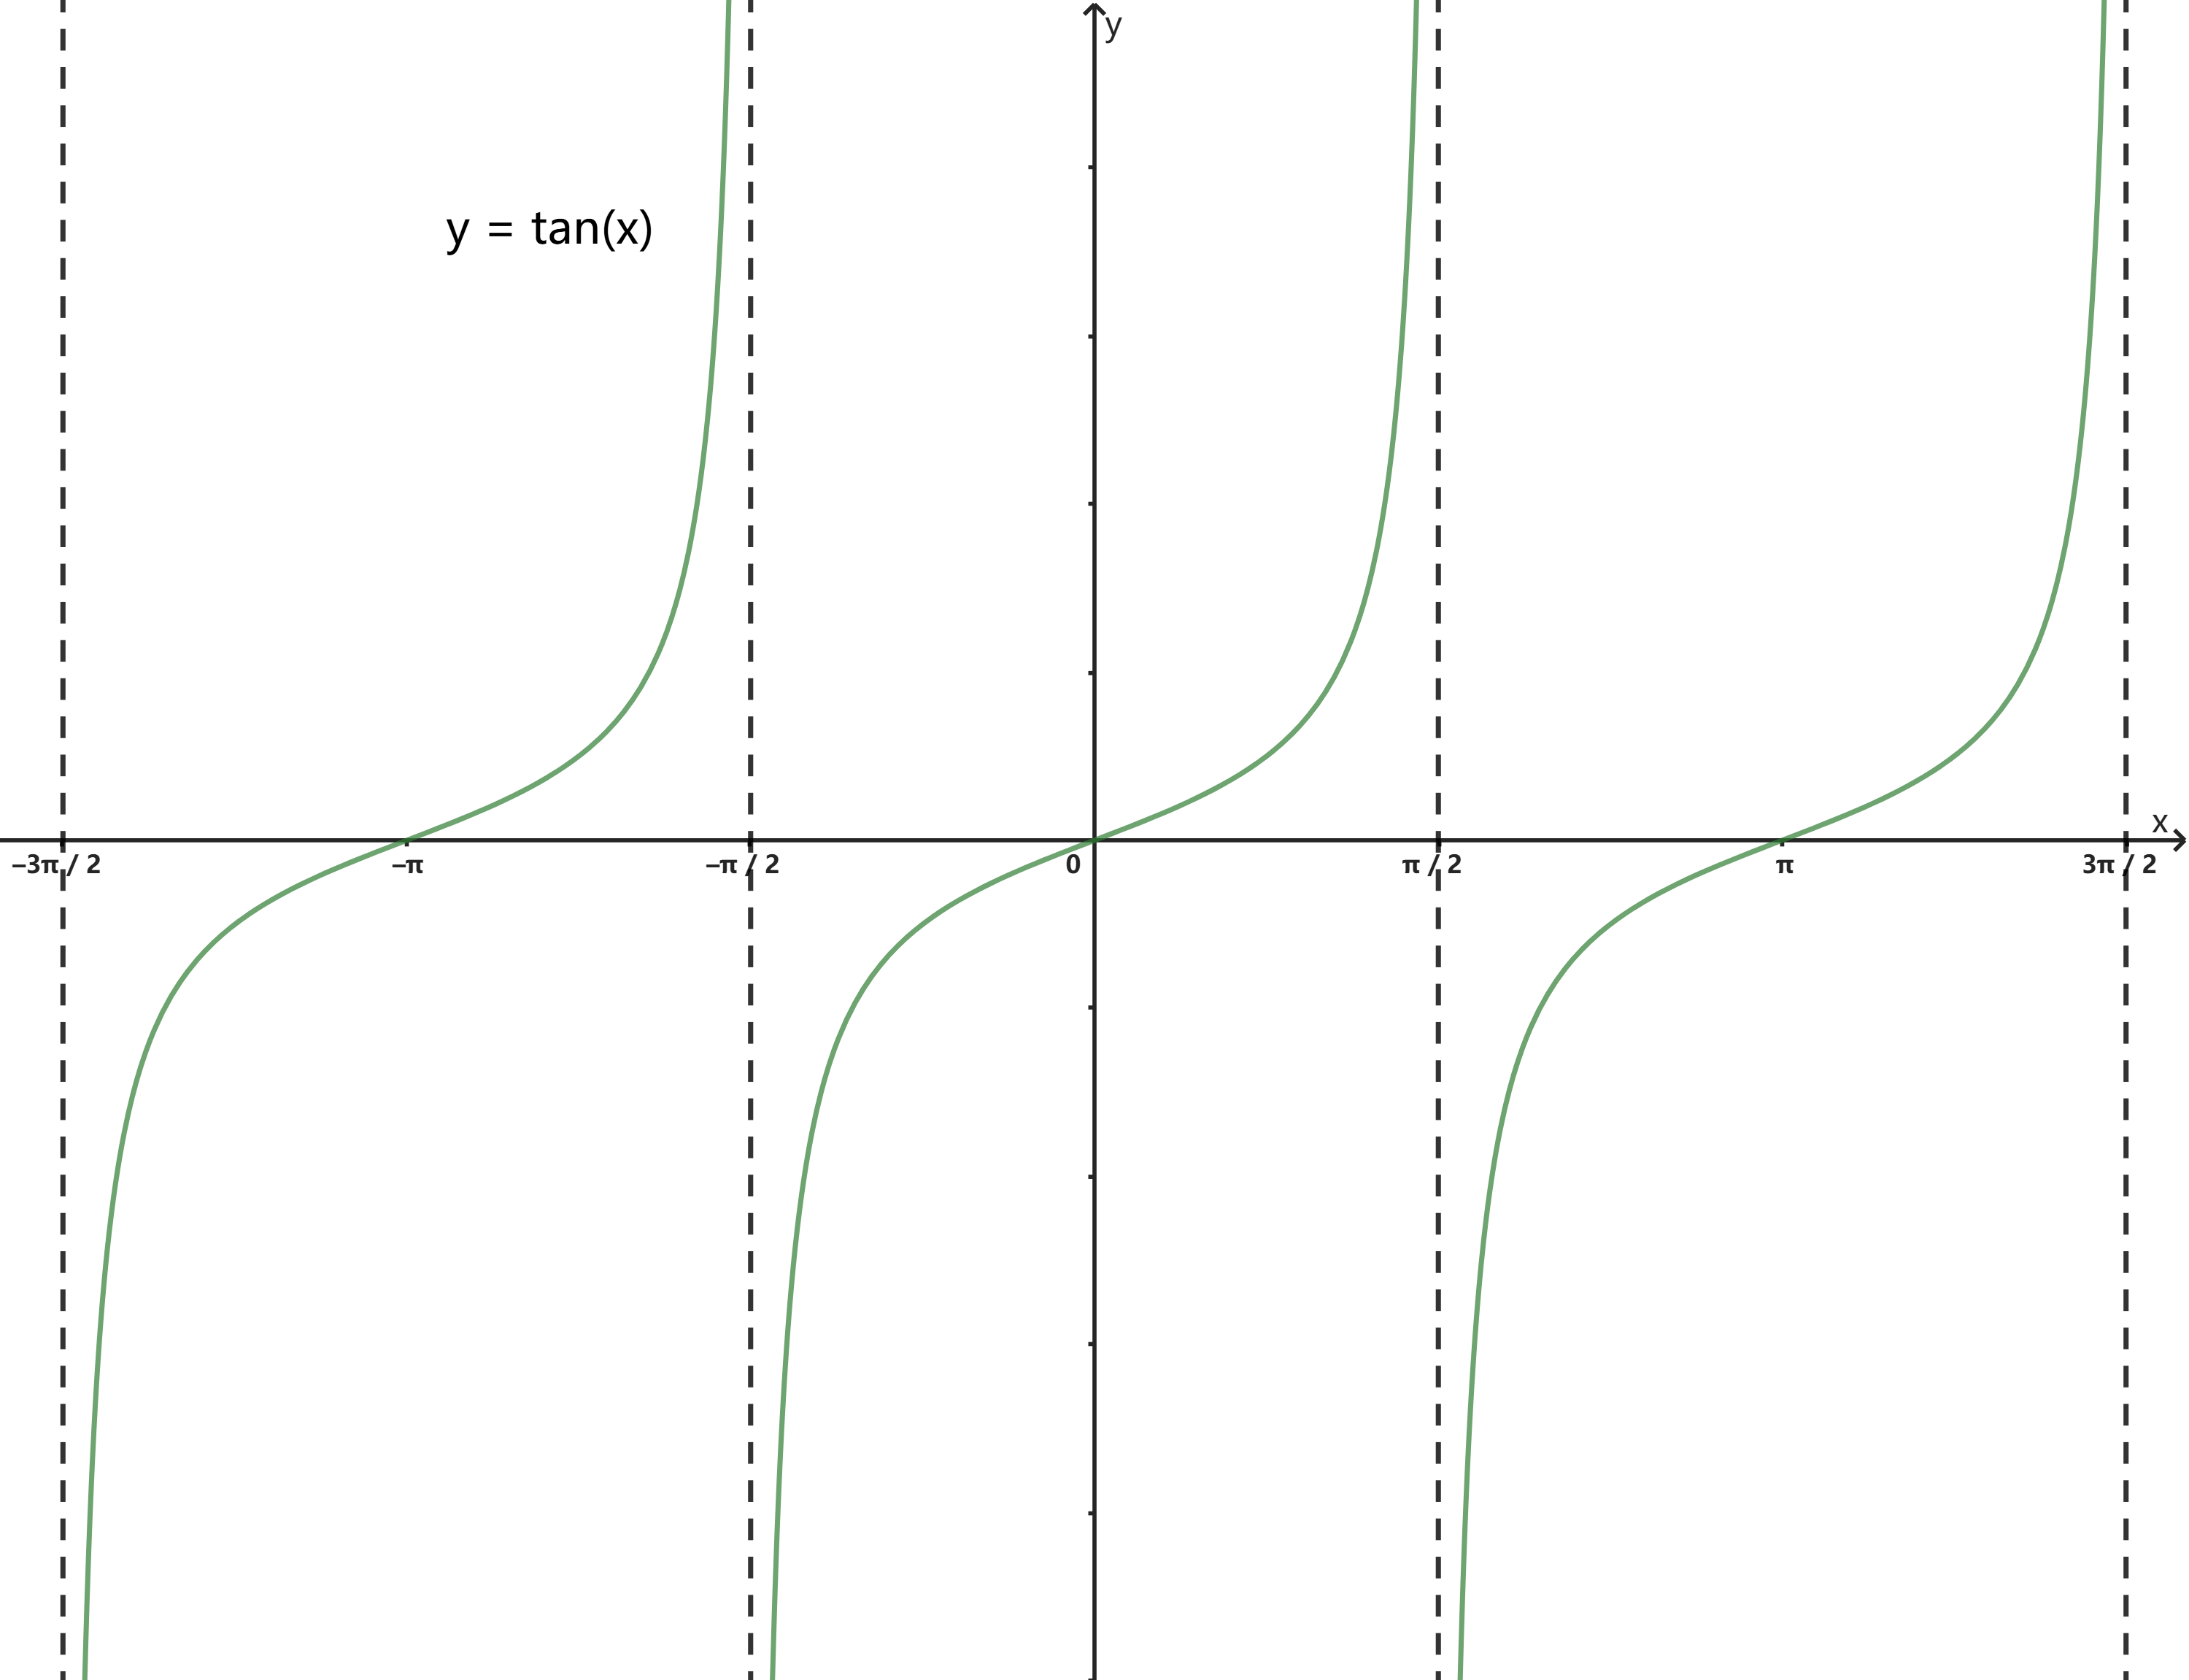
\includegraphics[width=\textwidth]{figure/tan_plot.png}}
    \caption{} \label{tan}
\end{minipage}
    \qquad
\begin{minipage}{0.4\linewidth}
    %\vspace{3pt}
    \centerline{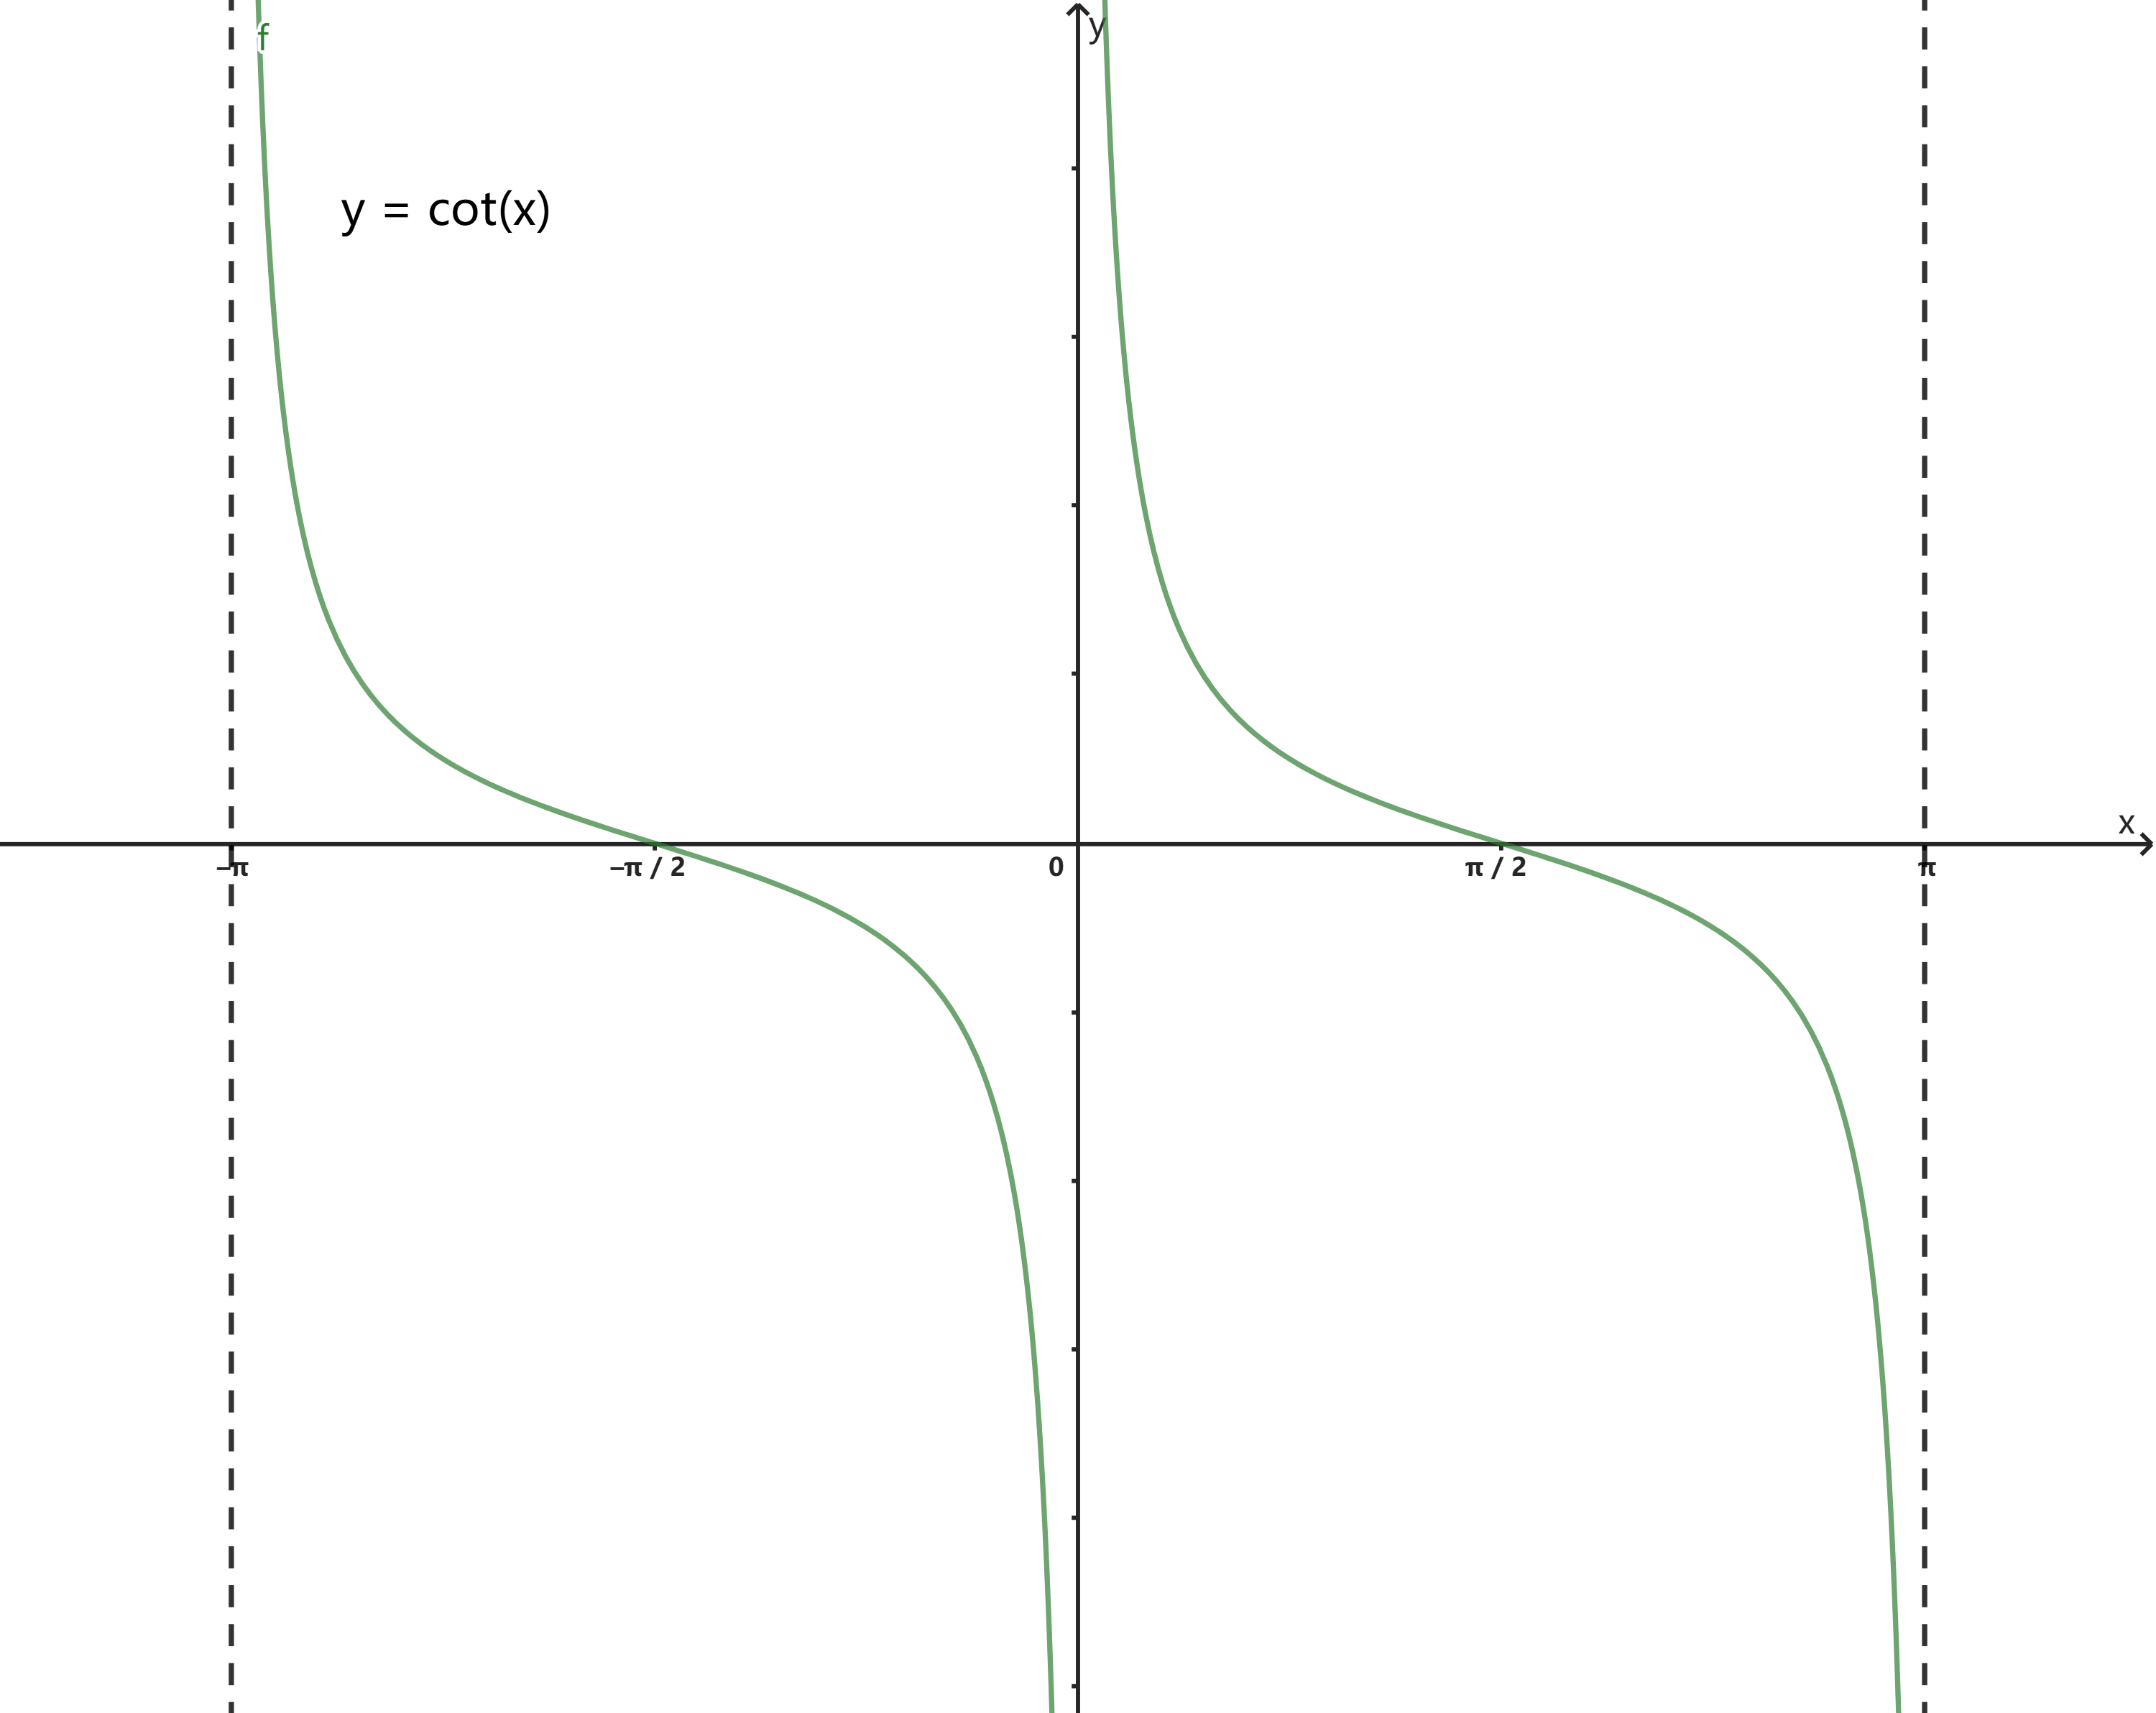
\includegraphics[width=\textwidth]{figure/cot_plot.png}}
    \caption{} \label{cot}
\end{minipage}
\end{figure}

\begin{note}
    \begin{enumerate}
        \item 定义域:$y=\tan x$的定义域为$x\neq k\pi+\dfrac{\pi}{2}(k\in Z)$的一切实数$x$;
        \vspace{2mm}

        $y=\cot x$的定义域为$x\neq k\pi(k\in Z)$的一切实数$x$。

        值域:$(-\infty,+\infty)$

        \item 奇偶性:$y=\tan x$和$y=\cot x$均为奇函数(在其定义域内)。

        \item 周期性:$y=\tan x$和$y=\cot x$均以$\pi$为最小正周期(在其定义域内)。
    \end{enumerate}
\end{note}
~\\

\textbf{正割函数与余割函数}

正割函数$y=\sec x$(见图\ref{sec}),余割函数$y=\csc x$(见图\ref{csc})
\begin{equation}
    \sec x = \dfrac{1}{\cos x}, \quad \csc x = \dfrac{1}{\sin x} \nonumber
\end{equation}

\begin{figure}[H]
\centering
\begin{minipage}{0.4\linewidth}
    \centerline{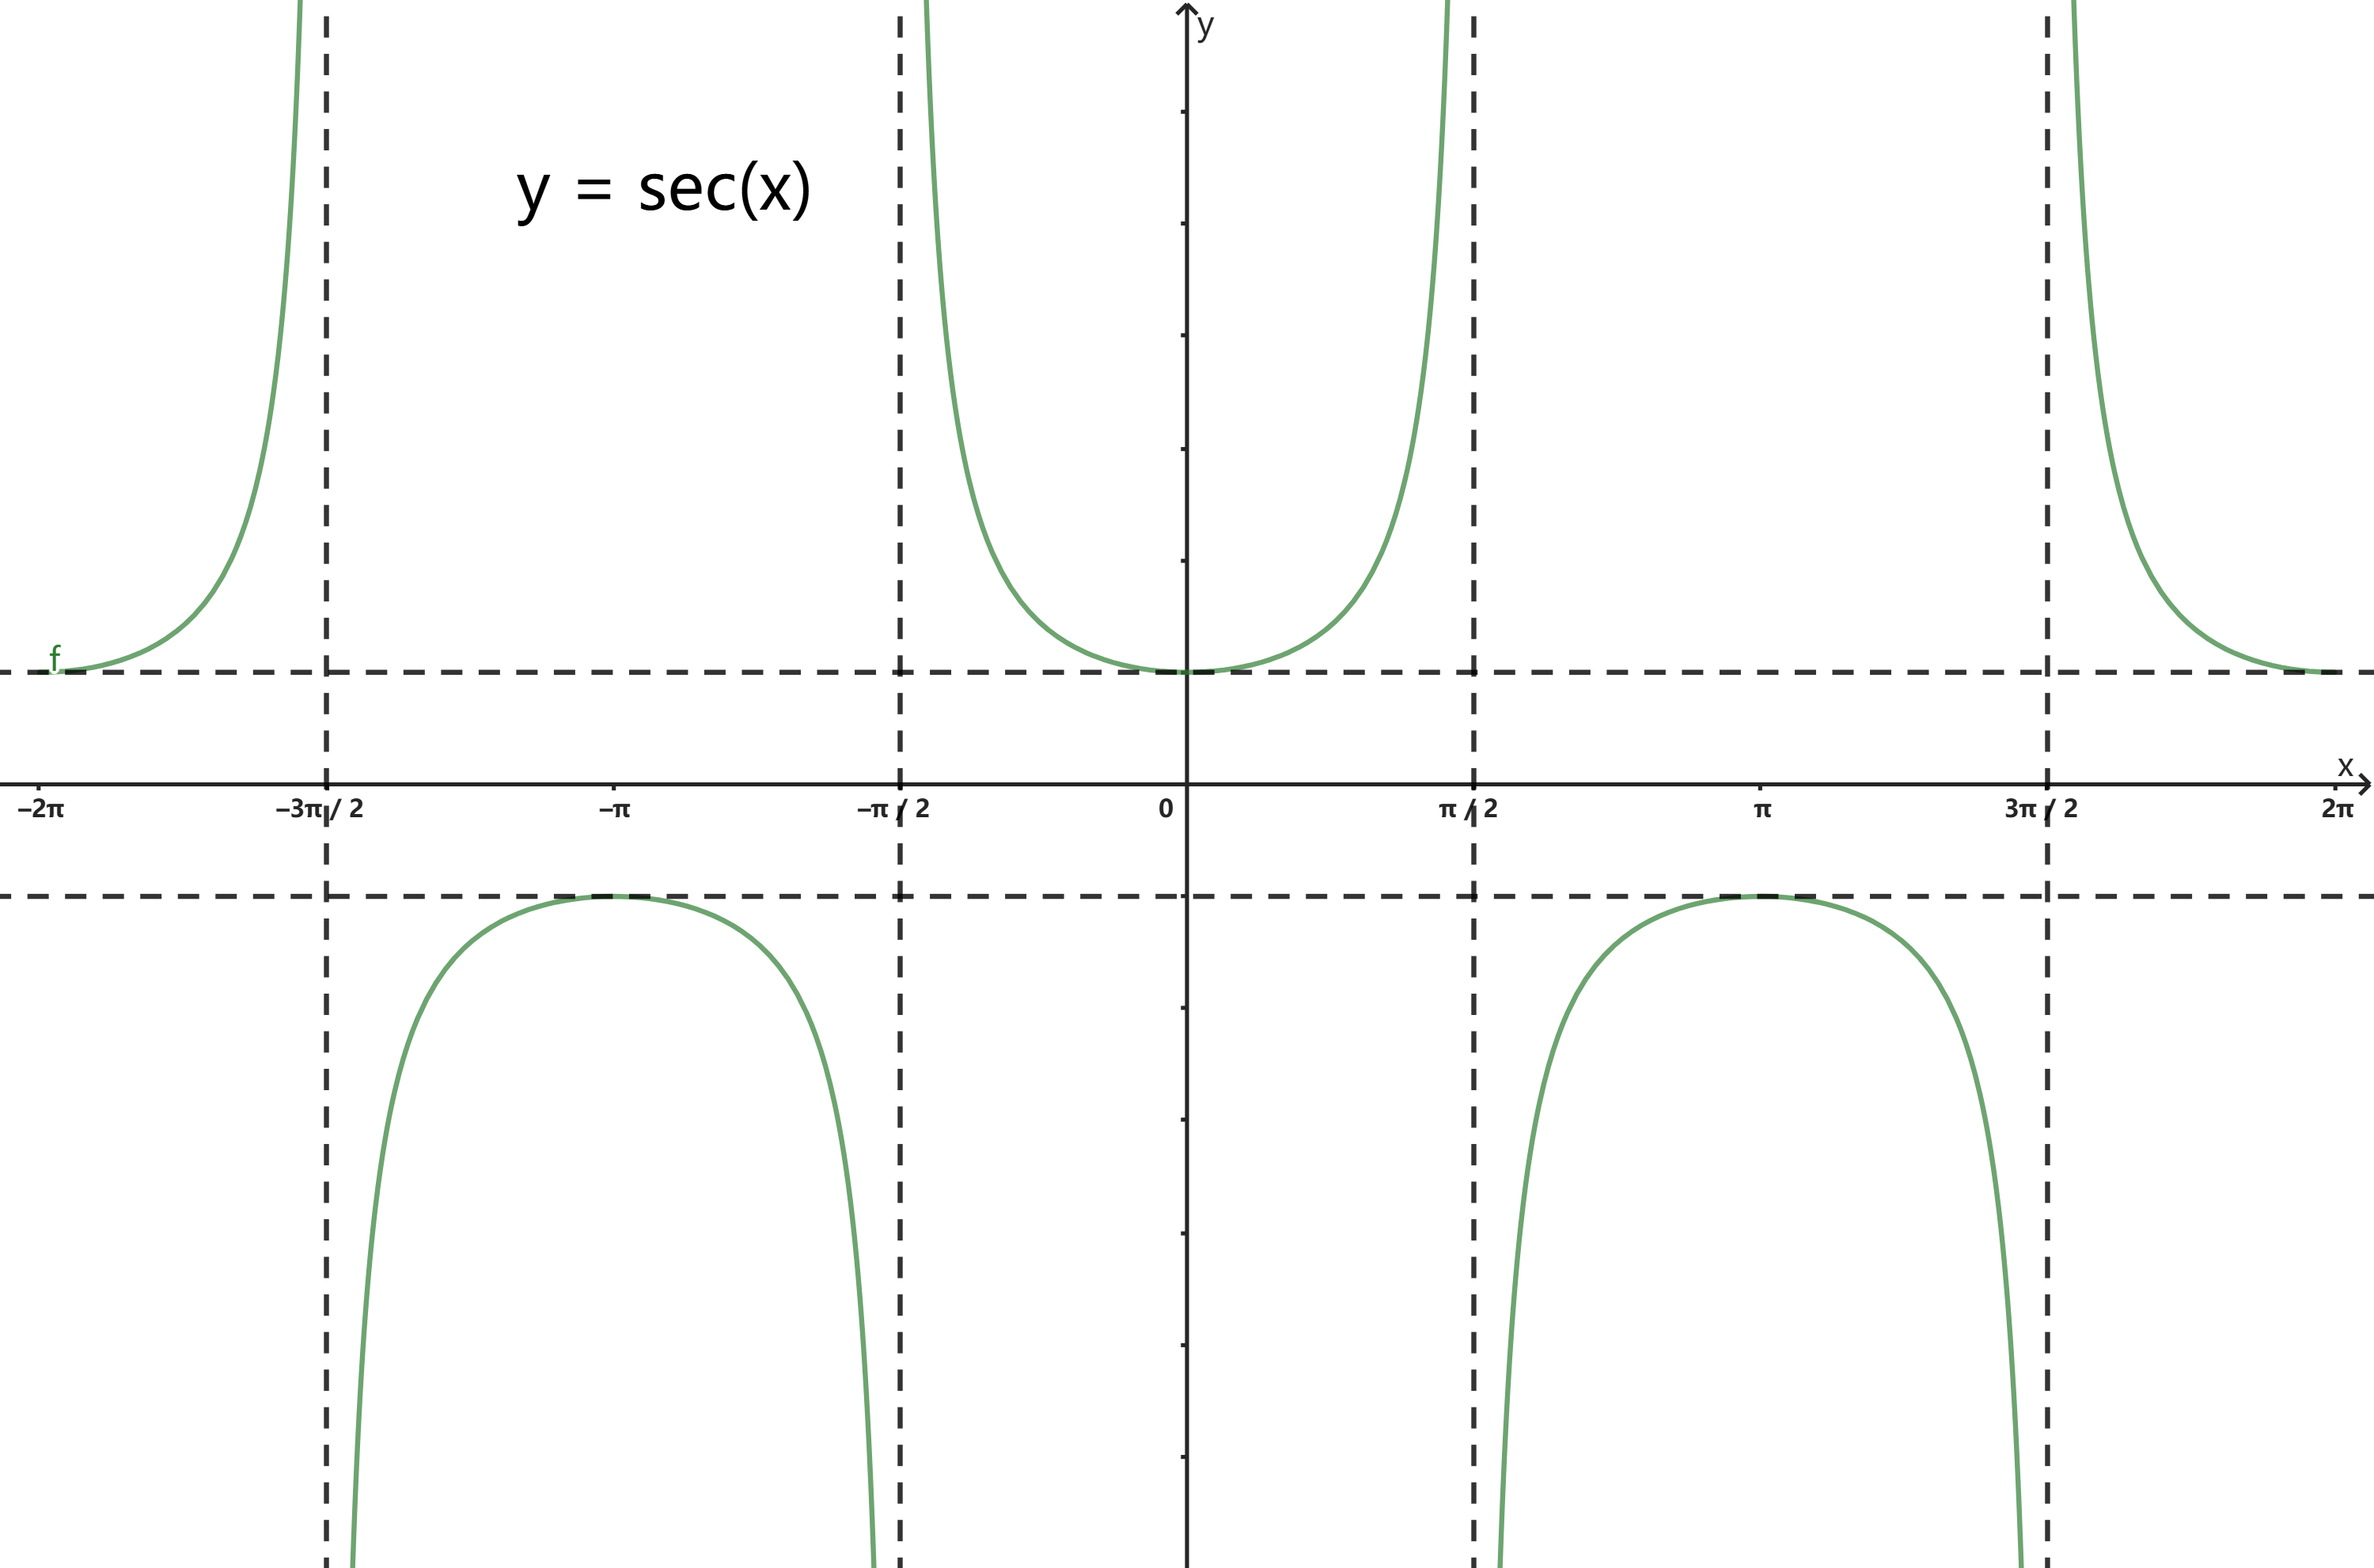
\includegraphics[width=\textwidth]{figure/sec_plot.png}}
    \caption{} \label{sec}
\end{minipage}
    \qquad
\begin{minipage}{0.4\linewidth}
    %\vspace{3pt}
    \centerline{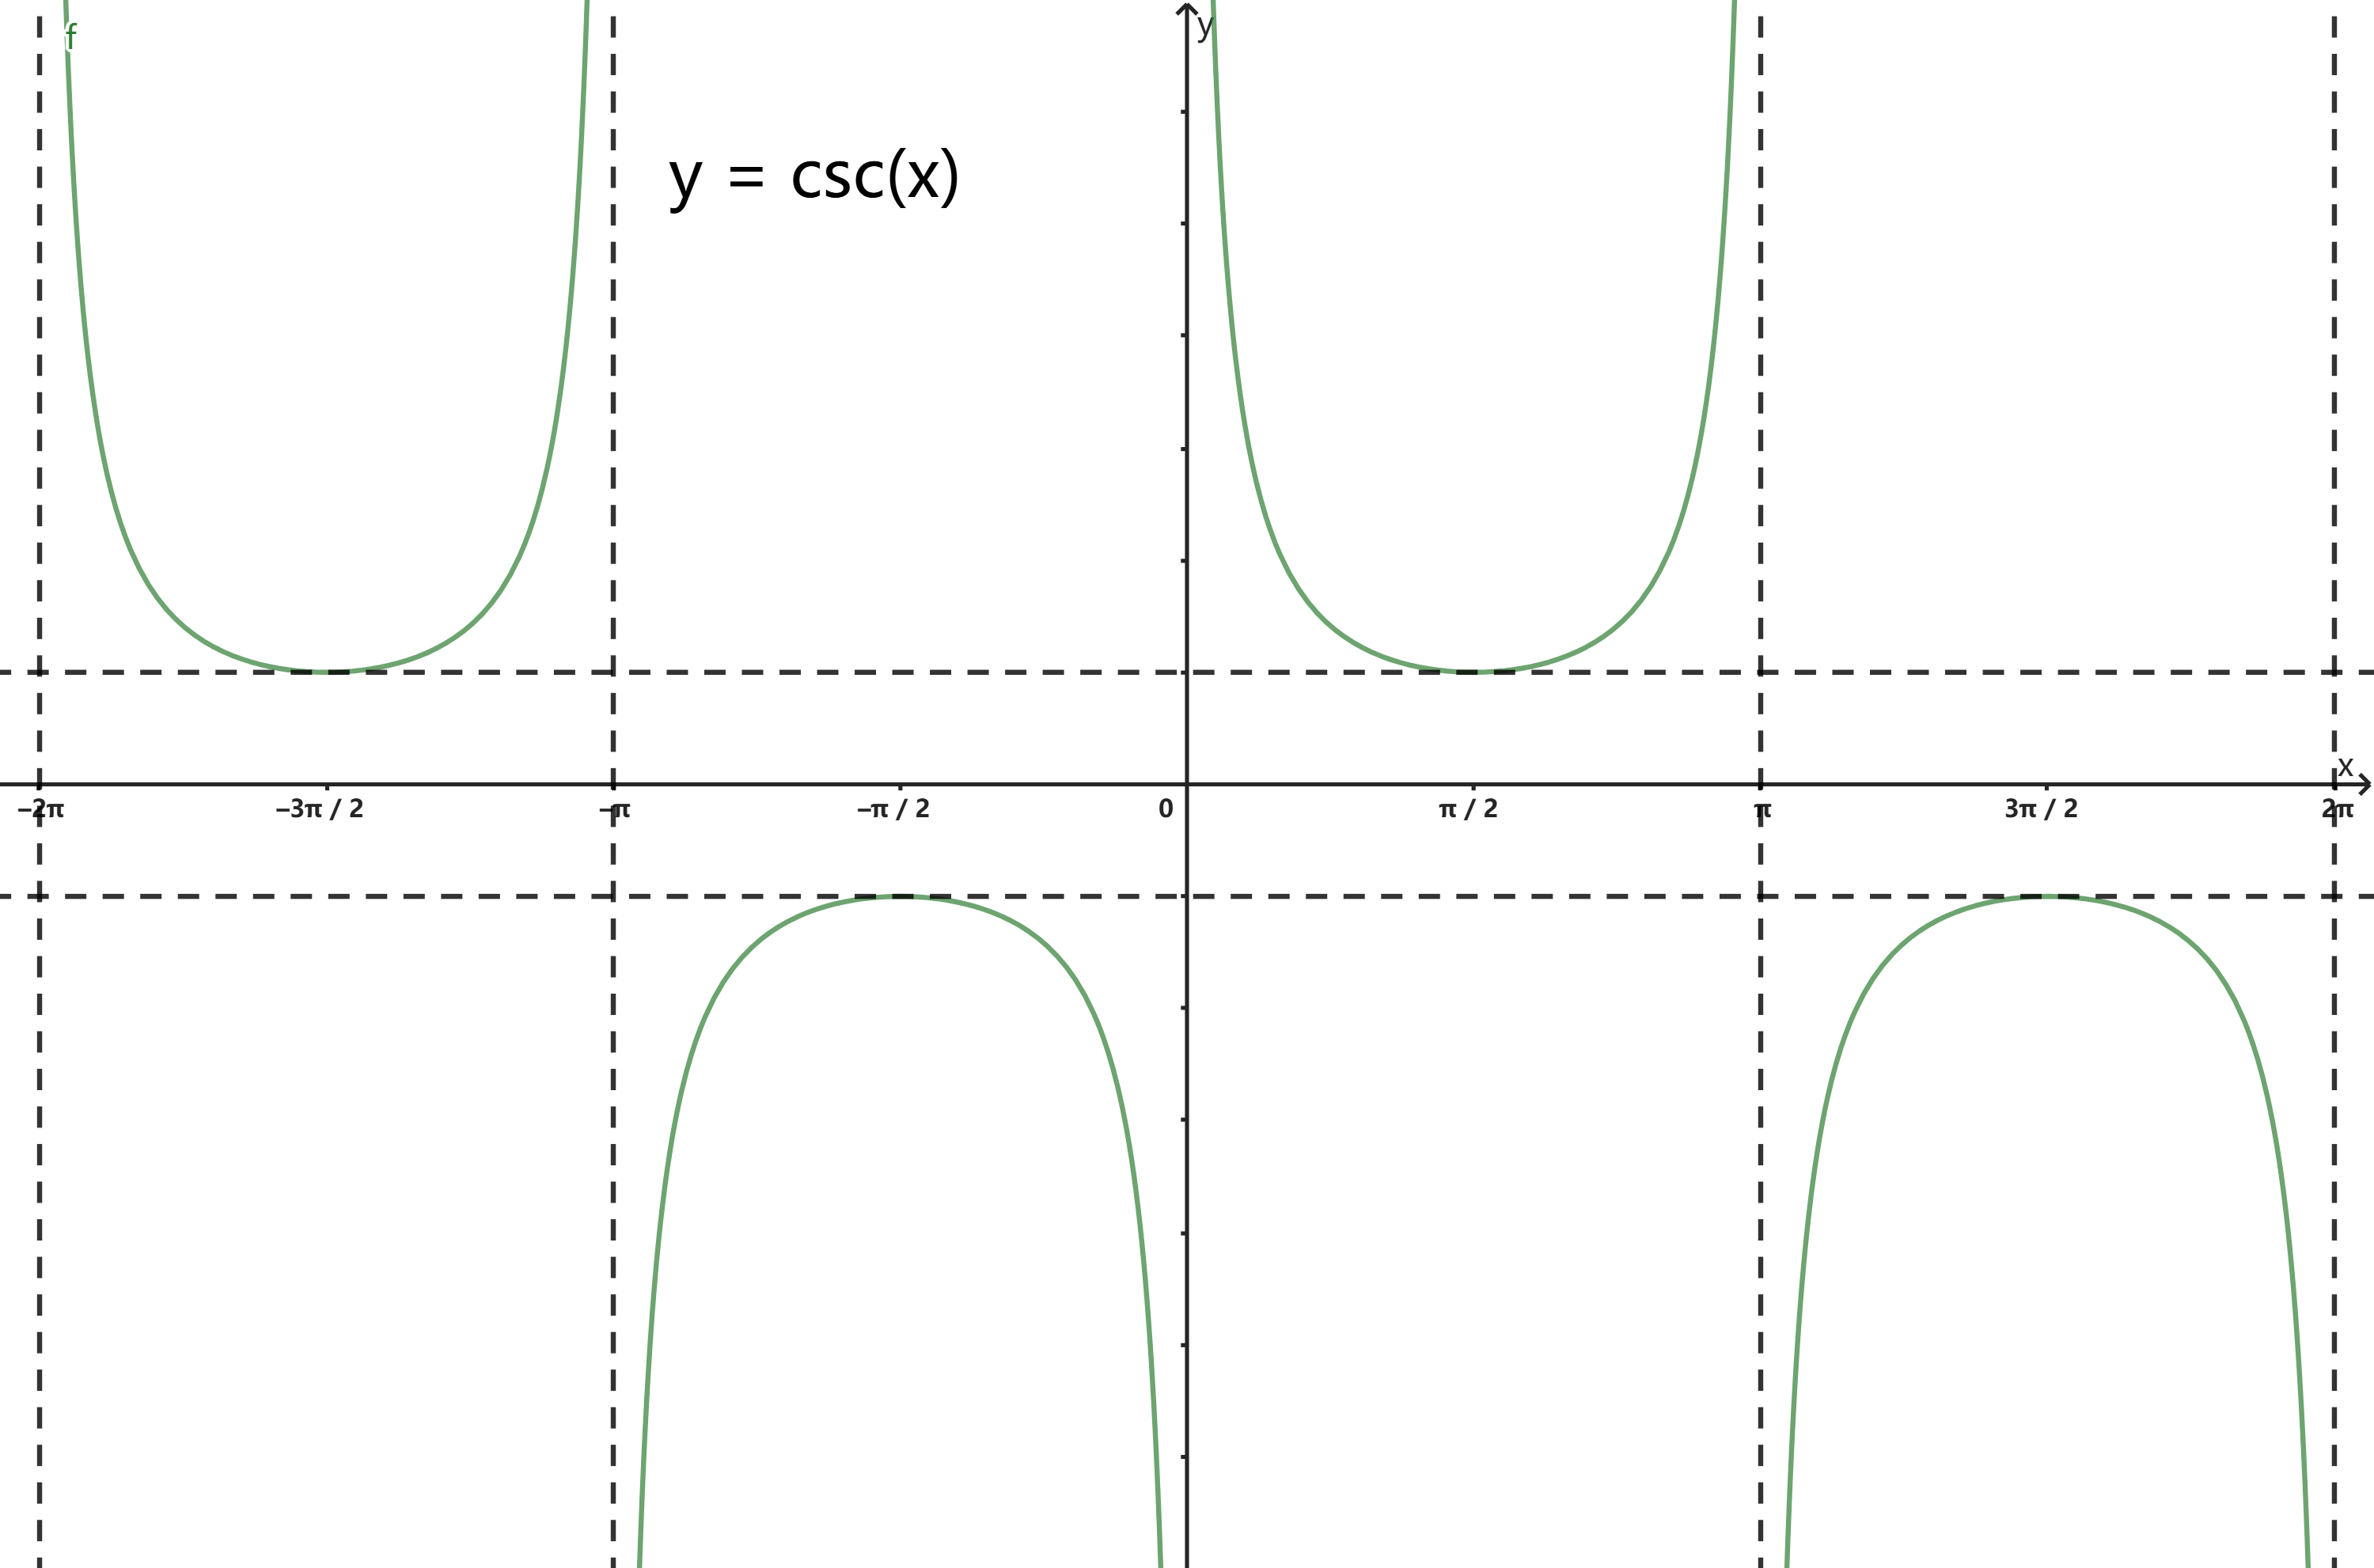
\includegraphics[width=\textwidth]{figure/csc_plot.png}}
    \caption{} \label{csc}
\end{minipage}
\end{figure}

\begin{note}
    \begin{enumerate}
        \item 定义域:$y=\sec x$的定义域为$x\neq k\pi+\dfrac{\pi}{2}(k\in Z)$的一切实数$x$;
        \vspace{2mm}

        $y=\csc x$的定义域为$x\neq k\pi(k\in Z)$的一切实数$x$。

        值域:$(-\infty,-1]\cup [1,+\infty)$

        \item 奇偶性:$y=\sec x$为偶函数,$y=\csc x$为奇函数(在其定义域内)。

        \item 周期性:$y=\sec x$和$y=\csc x$均以$2\pi$为最小正周期(在其定义域内)。
    \end{enumerate}
\end{note}

\subsection{反三角函数函数图像及性质}
\textbf{反正弦函数与反余弦函数}

反正弦函数$y=\arcsin x$(见图\ref{arcsin}),反余弦函数$y=\arccos x$(见图\ref{arccos})
\begin{figure}[H]
\centering
\begin{minipage}{0.4\linewidth}
    \centerline{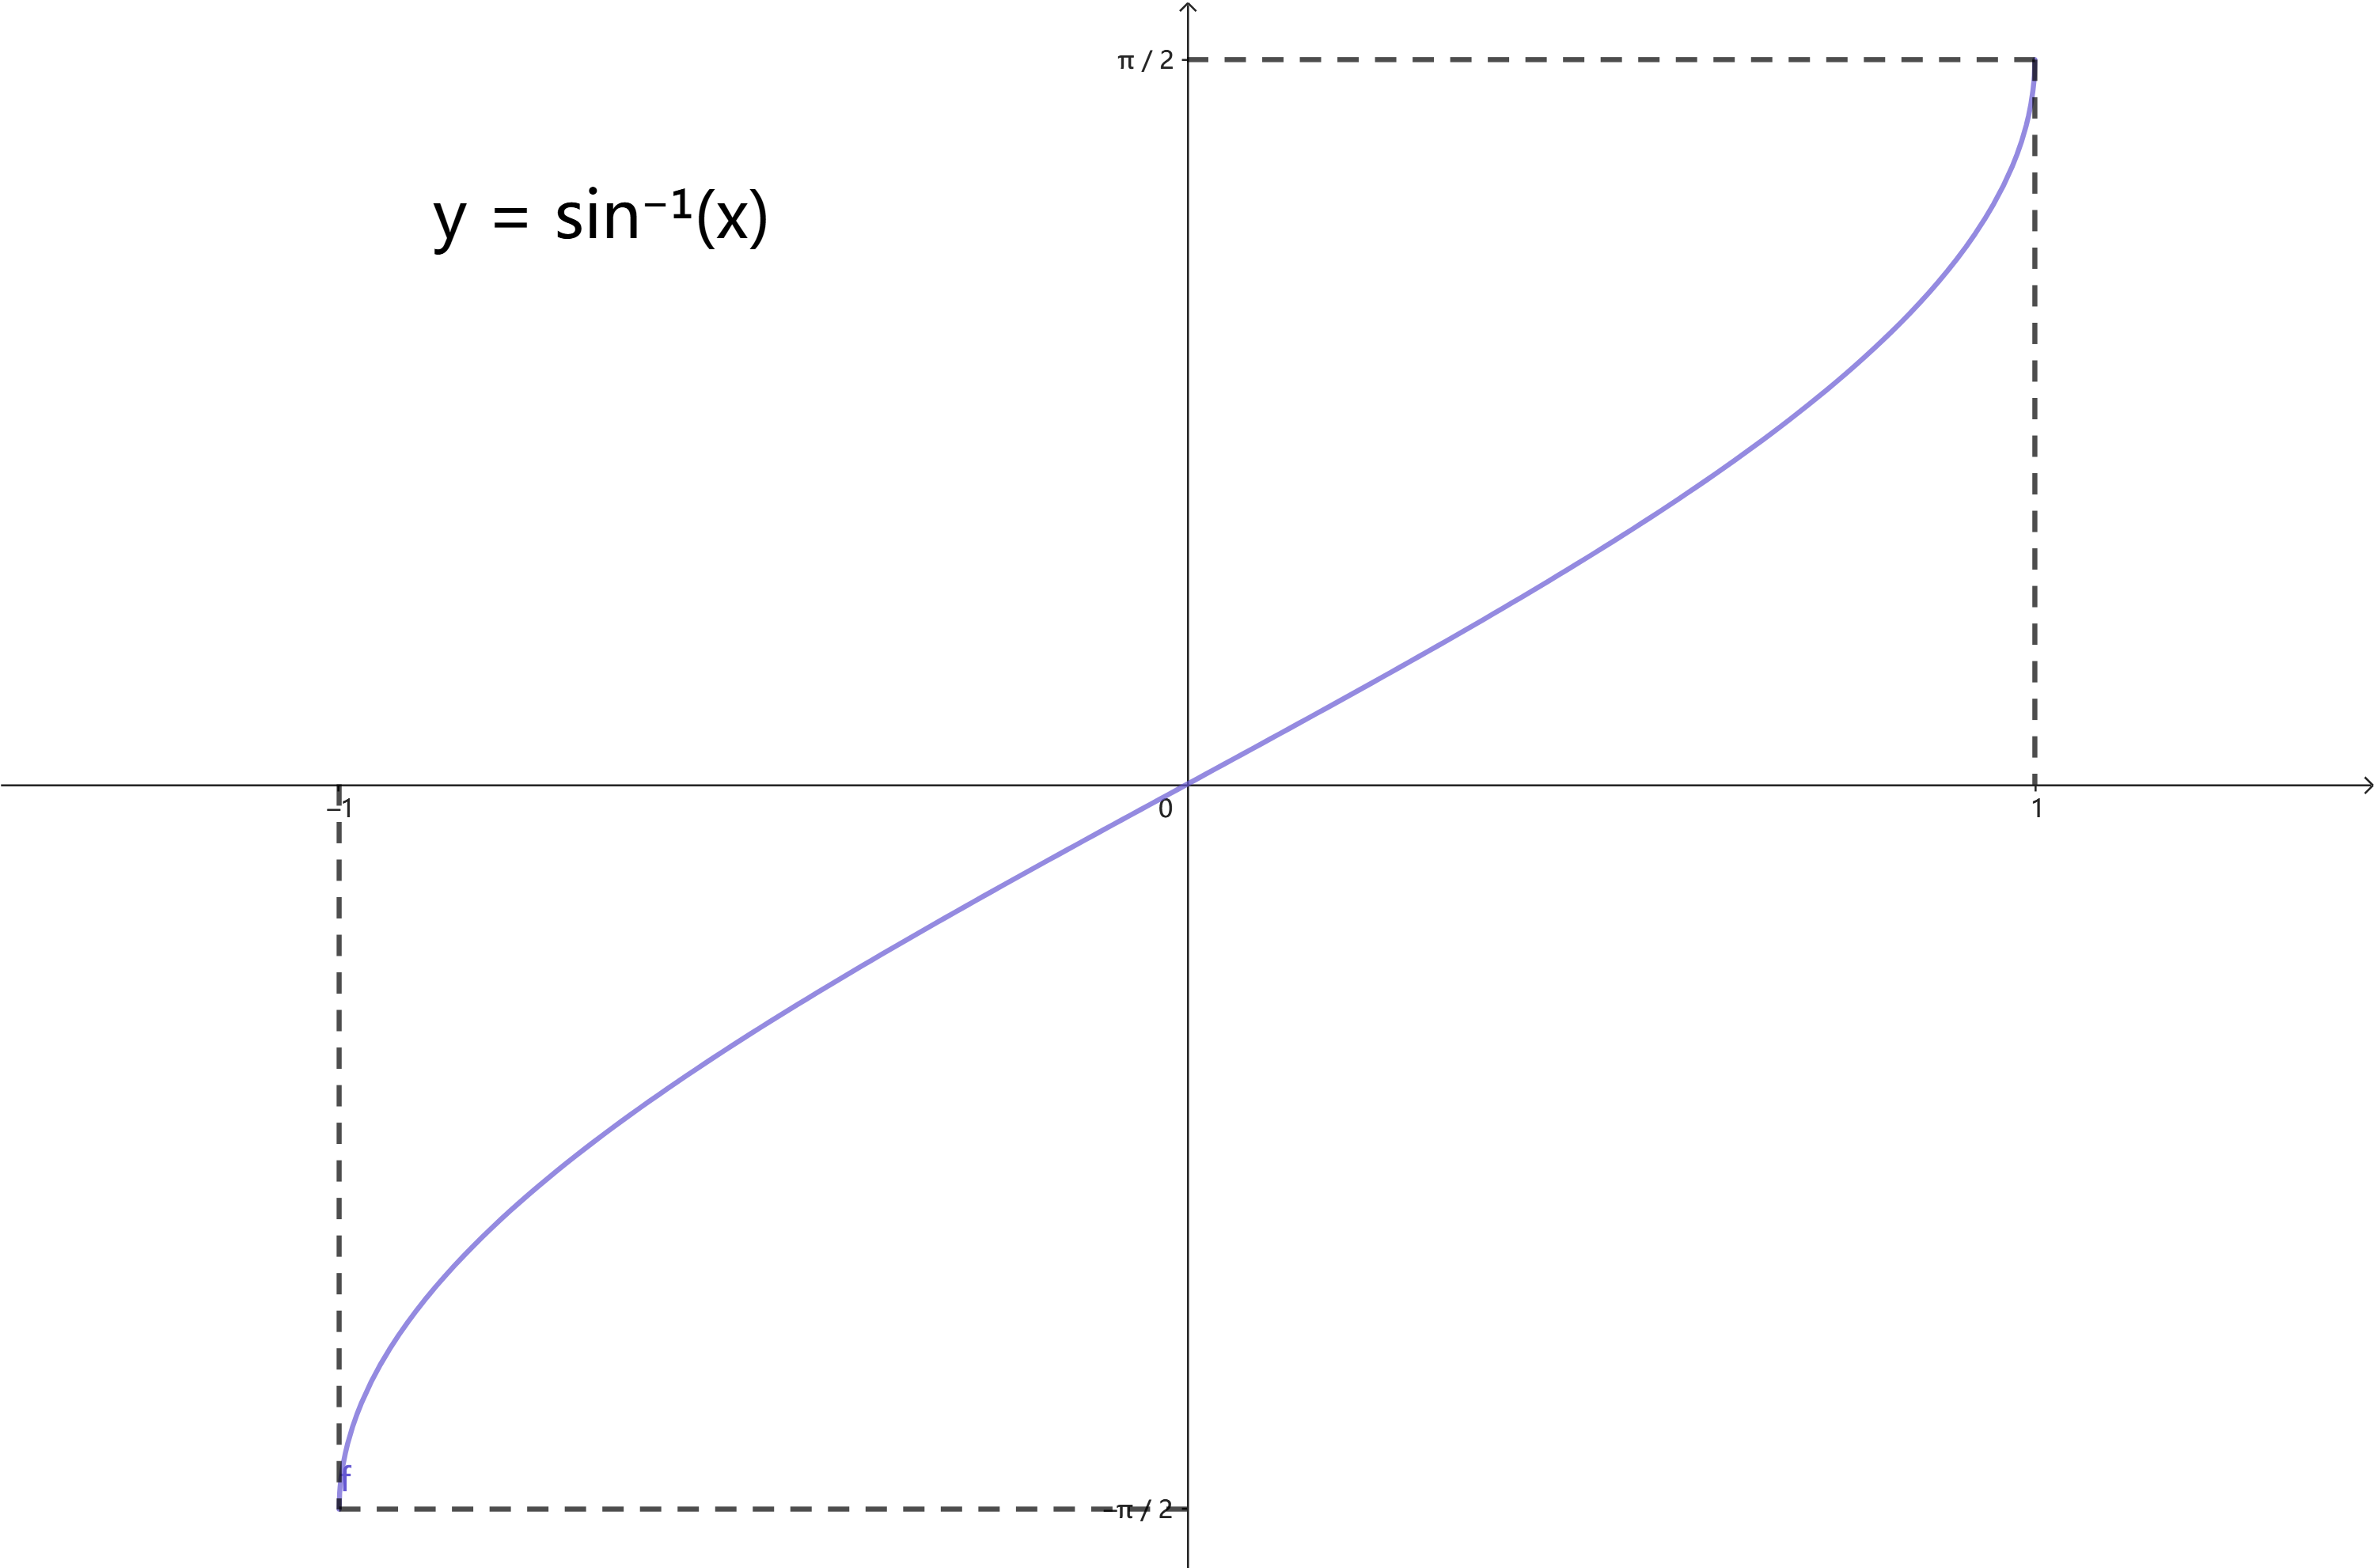
\includegraphics[width=\textwidth]{figure/arcsin_plot.png}}
    \caption{} \label{arcsin}
\end{minipage}
    \qquad
\begin{minipage}{0.4\linewidth}
    %\vspace{3pt}
    \centerline{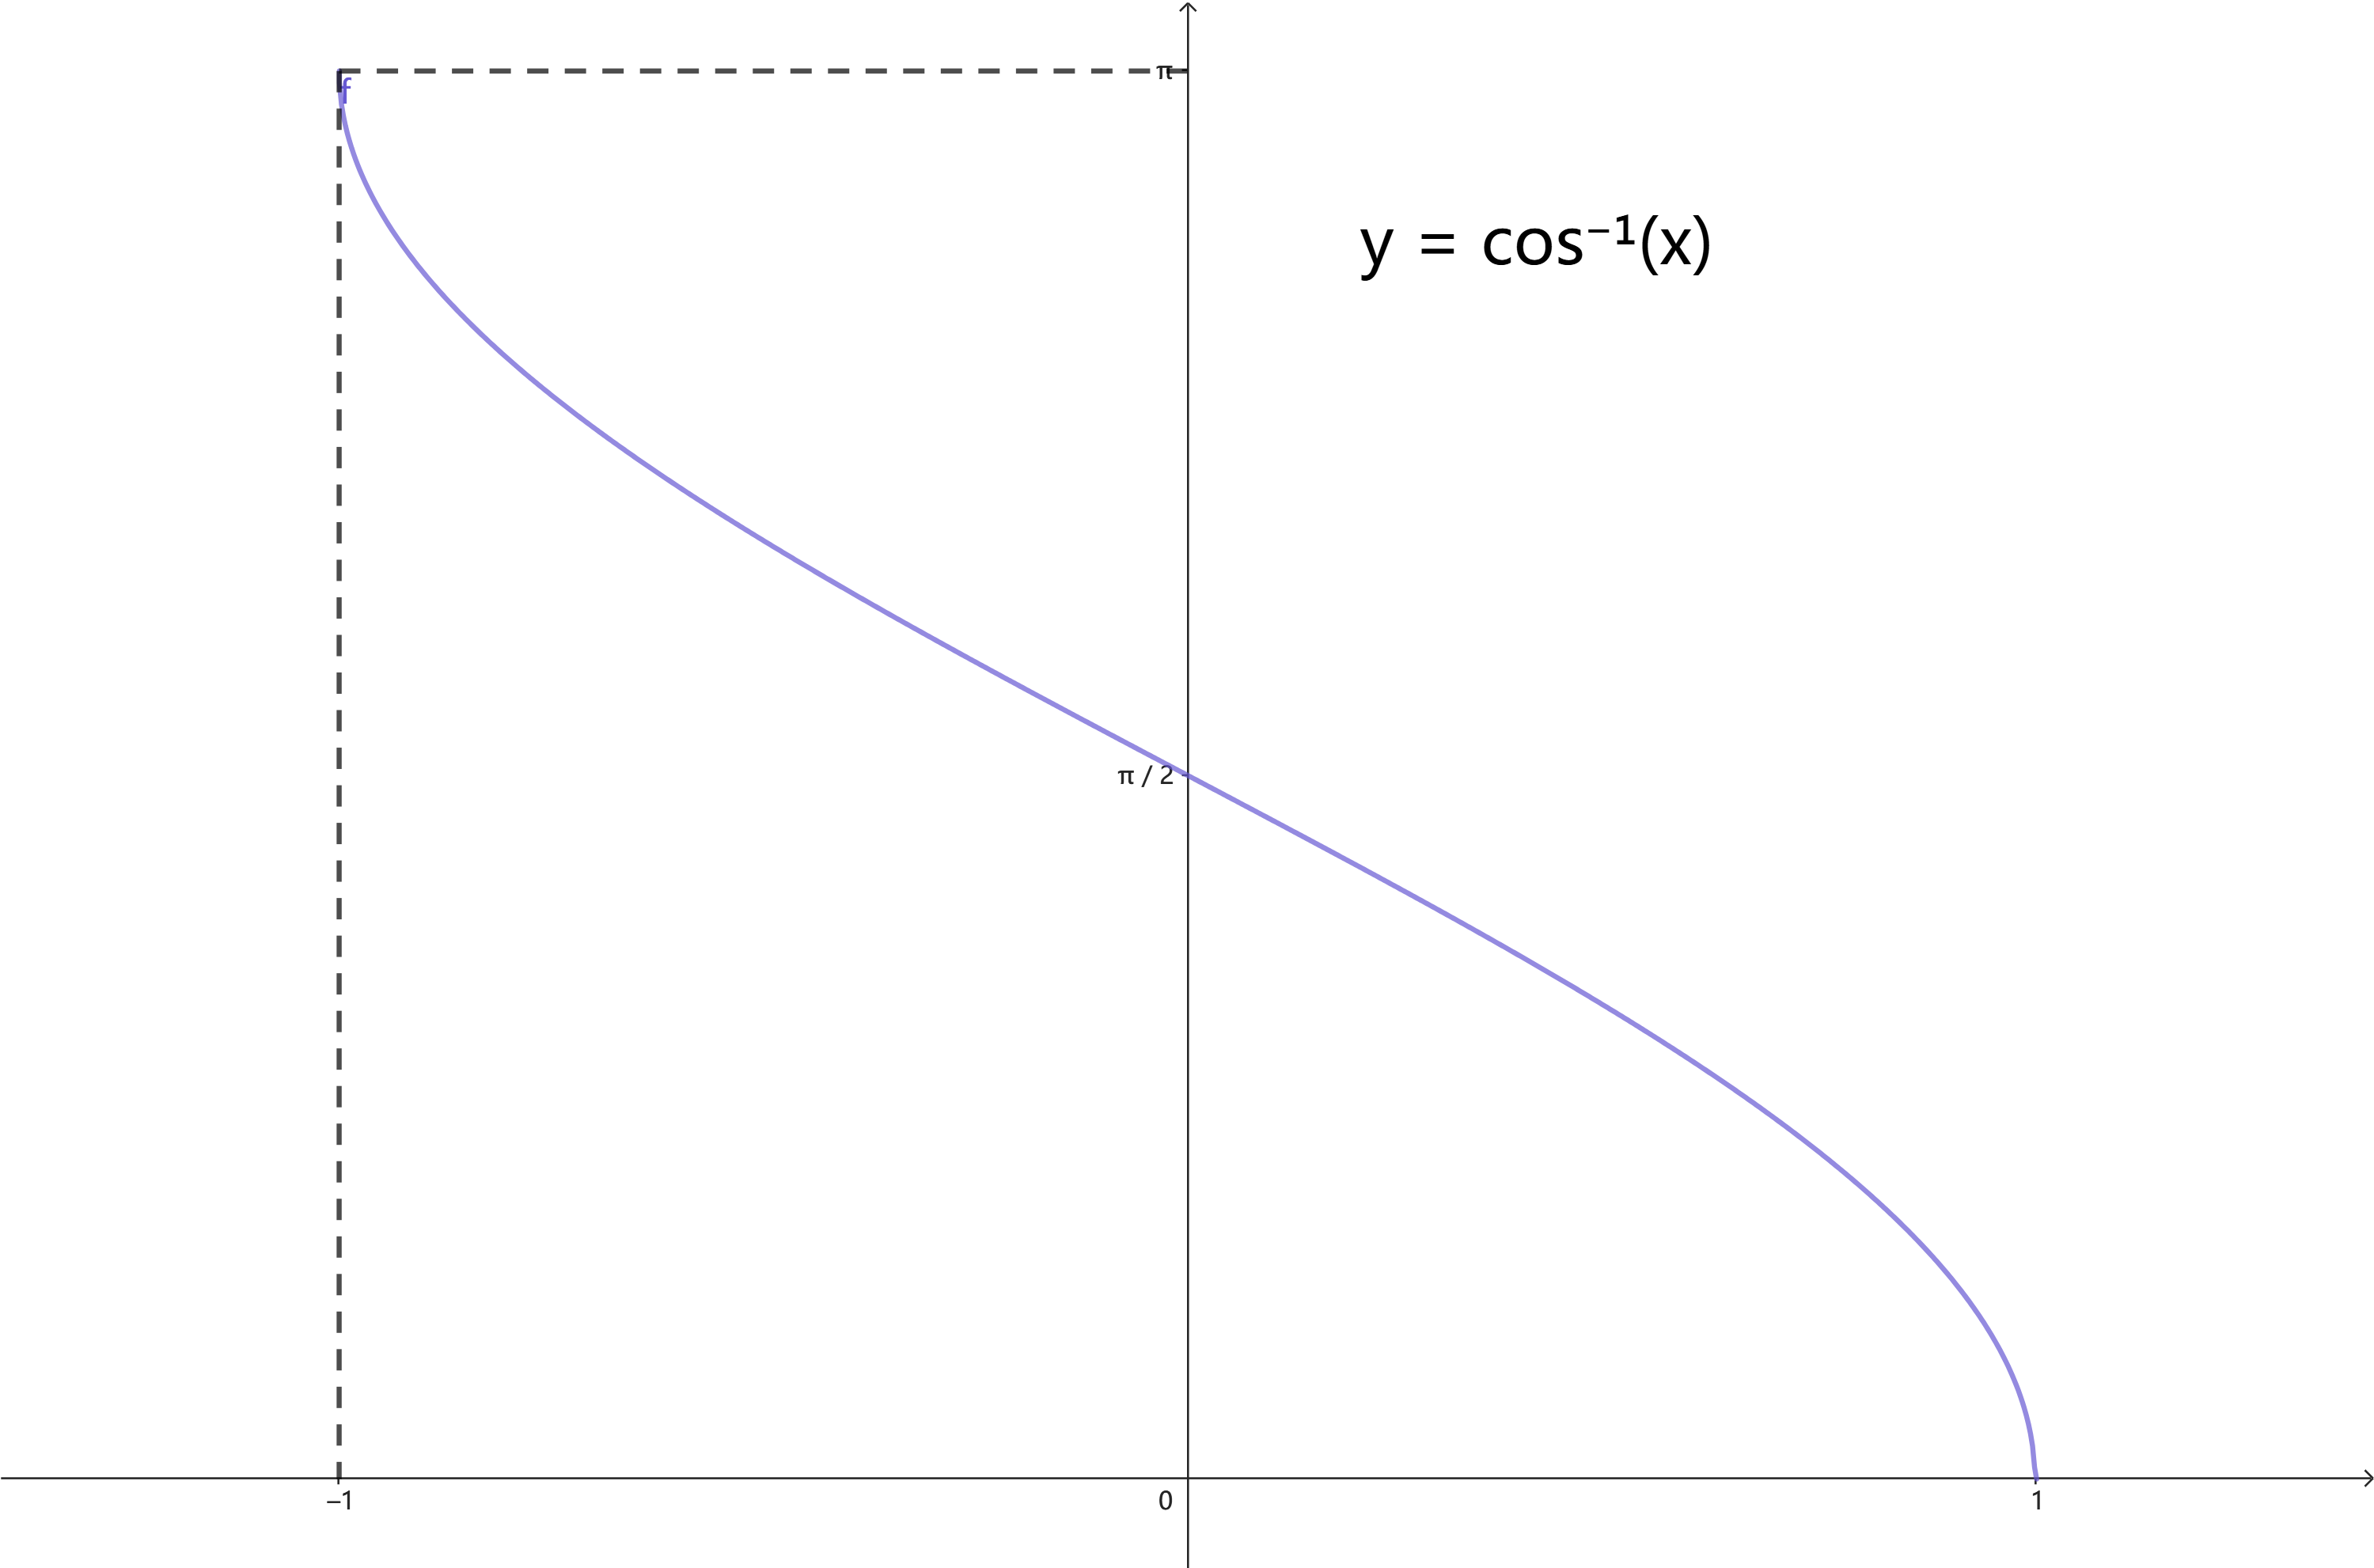
\includegraphics[width=\textwidth]{figure/arccos_plot.png}}
    \caption{} \label{arccos}
\end{minipage}
\end{figure}

$y=\arcsin x$是$y=\sin x\left(-\dfrac{\pi}{2}\leq x\leq \dfrac{\pi}{2}\right)$的反函数,$y=\arccos x$是$y=\cos x(0\leq x\leq \pi)$的反函数

\begin{note}
    \begin{enumerate}
        \item 定义域:[-1,1]

        值域:$y=\arcsin x$的值域为$\left[-\dfrac{\pi}{2},\dfrac{\pi}{2}\right]$,$y=\arccos x$的值域为$[0,\pi]$。

        \item 单调性:$y=\arcsin x$单调增加,$y=\arccos x$单调减少。

        \item 奇偶性:$y=\arcsin x$为奇函数(在其定义域内)。

        \item 有界性:两个函数在其定义域内有界,$-\dfrac{\pi}{2}\leq \arcsin x\leq \dfrac{\pi}{2}, 0\leq \arccos x\leq\pi$

        \item 性质:$\arcsin x+\arccos x = \dfrac{\pi}{2}(-1\leq x \leq 1)$
        \begin{proof}
            令$f(x)=\arcsin x+\arccos x,-1\leq x \leq 1$,则$f'(x)=\dfrac{1}{\sqrt{1-x^2}}-\dfrac{1}{\sqrt{1-x^2}}=0$,于是$f(x)=C$(常数),又$f(0)=\dfrac{\pi}{2}$,故$f(x)=\dfrac{\pi}{2}$,证毕。
        \end{proof}

        \item 特殊函数值:
        \begin{equation}
        \begin{aligned}
            &
            \arcsin 0 = 0, \quad \arcsin \dfrac{1}{2} = \dfrac{\pi}{6}, \quad \arcsin \dfrac{\sqrt{2}}{2} = \dfrac{\pi}{4}, \quad \arcsin \dfrac{\sqrt{3}}{2} = \dfrac{\pi}{3}, \quad \arcsin 1 = \dfrac{\pi}{2} \\
            &
            \arccos 1 = 0, \quad \arccos \dfrac{\sqrt{3}}{2} = \dfrac{\pi}{6}, \quad \arccos \dfrac{\sqrt{2}}{2} = \dfrac{\pi}{4}, \quad \arccos \dfrac{1}{2} = \dfrac{\pi}{3}, \quad \arccos 0 = \dfrac{\pi}{2}
        \end{aligned}    \nonumber
        \end{equation}
    \end{enumerate}
\end{note}
~\\

\textbf{反正切函数与反余切函数}

反正弦函数$y=\arctan x$(见图\ref{arctan}),反余弦函数$y=\arccot x$(见图\ref{arccot})
\begin{figure}[H]
\centering
\begin{minipage}{0.4\linewidth}
    \centerline{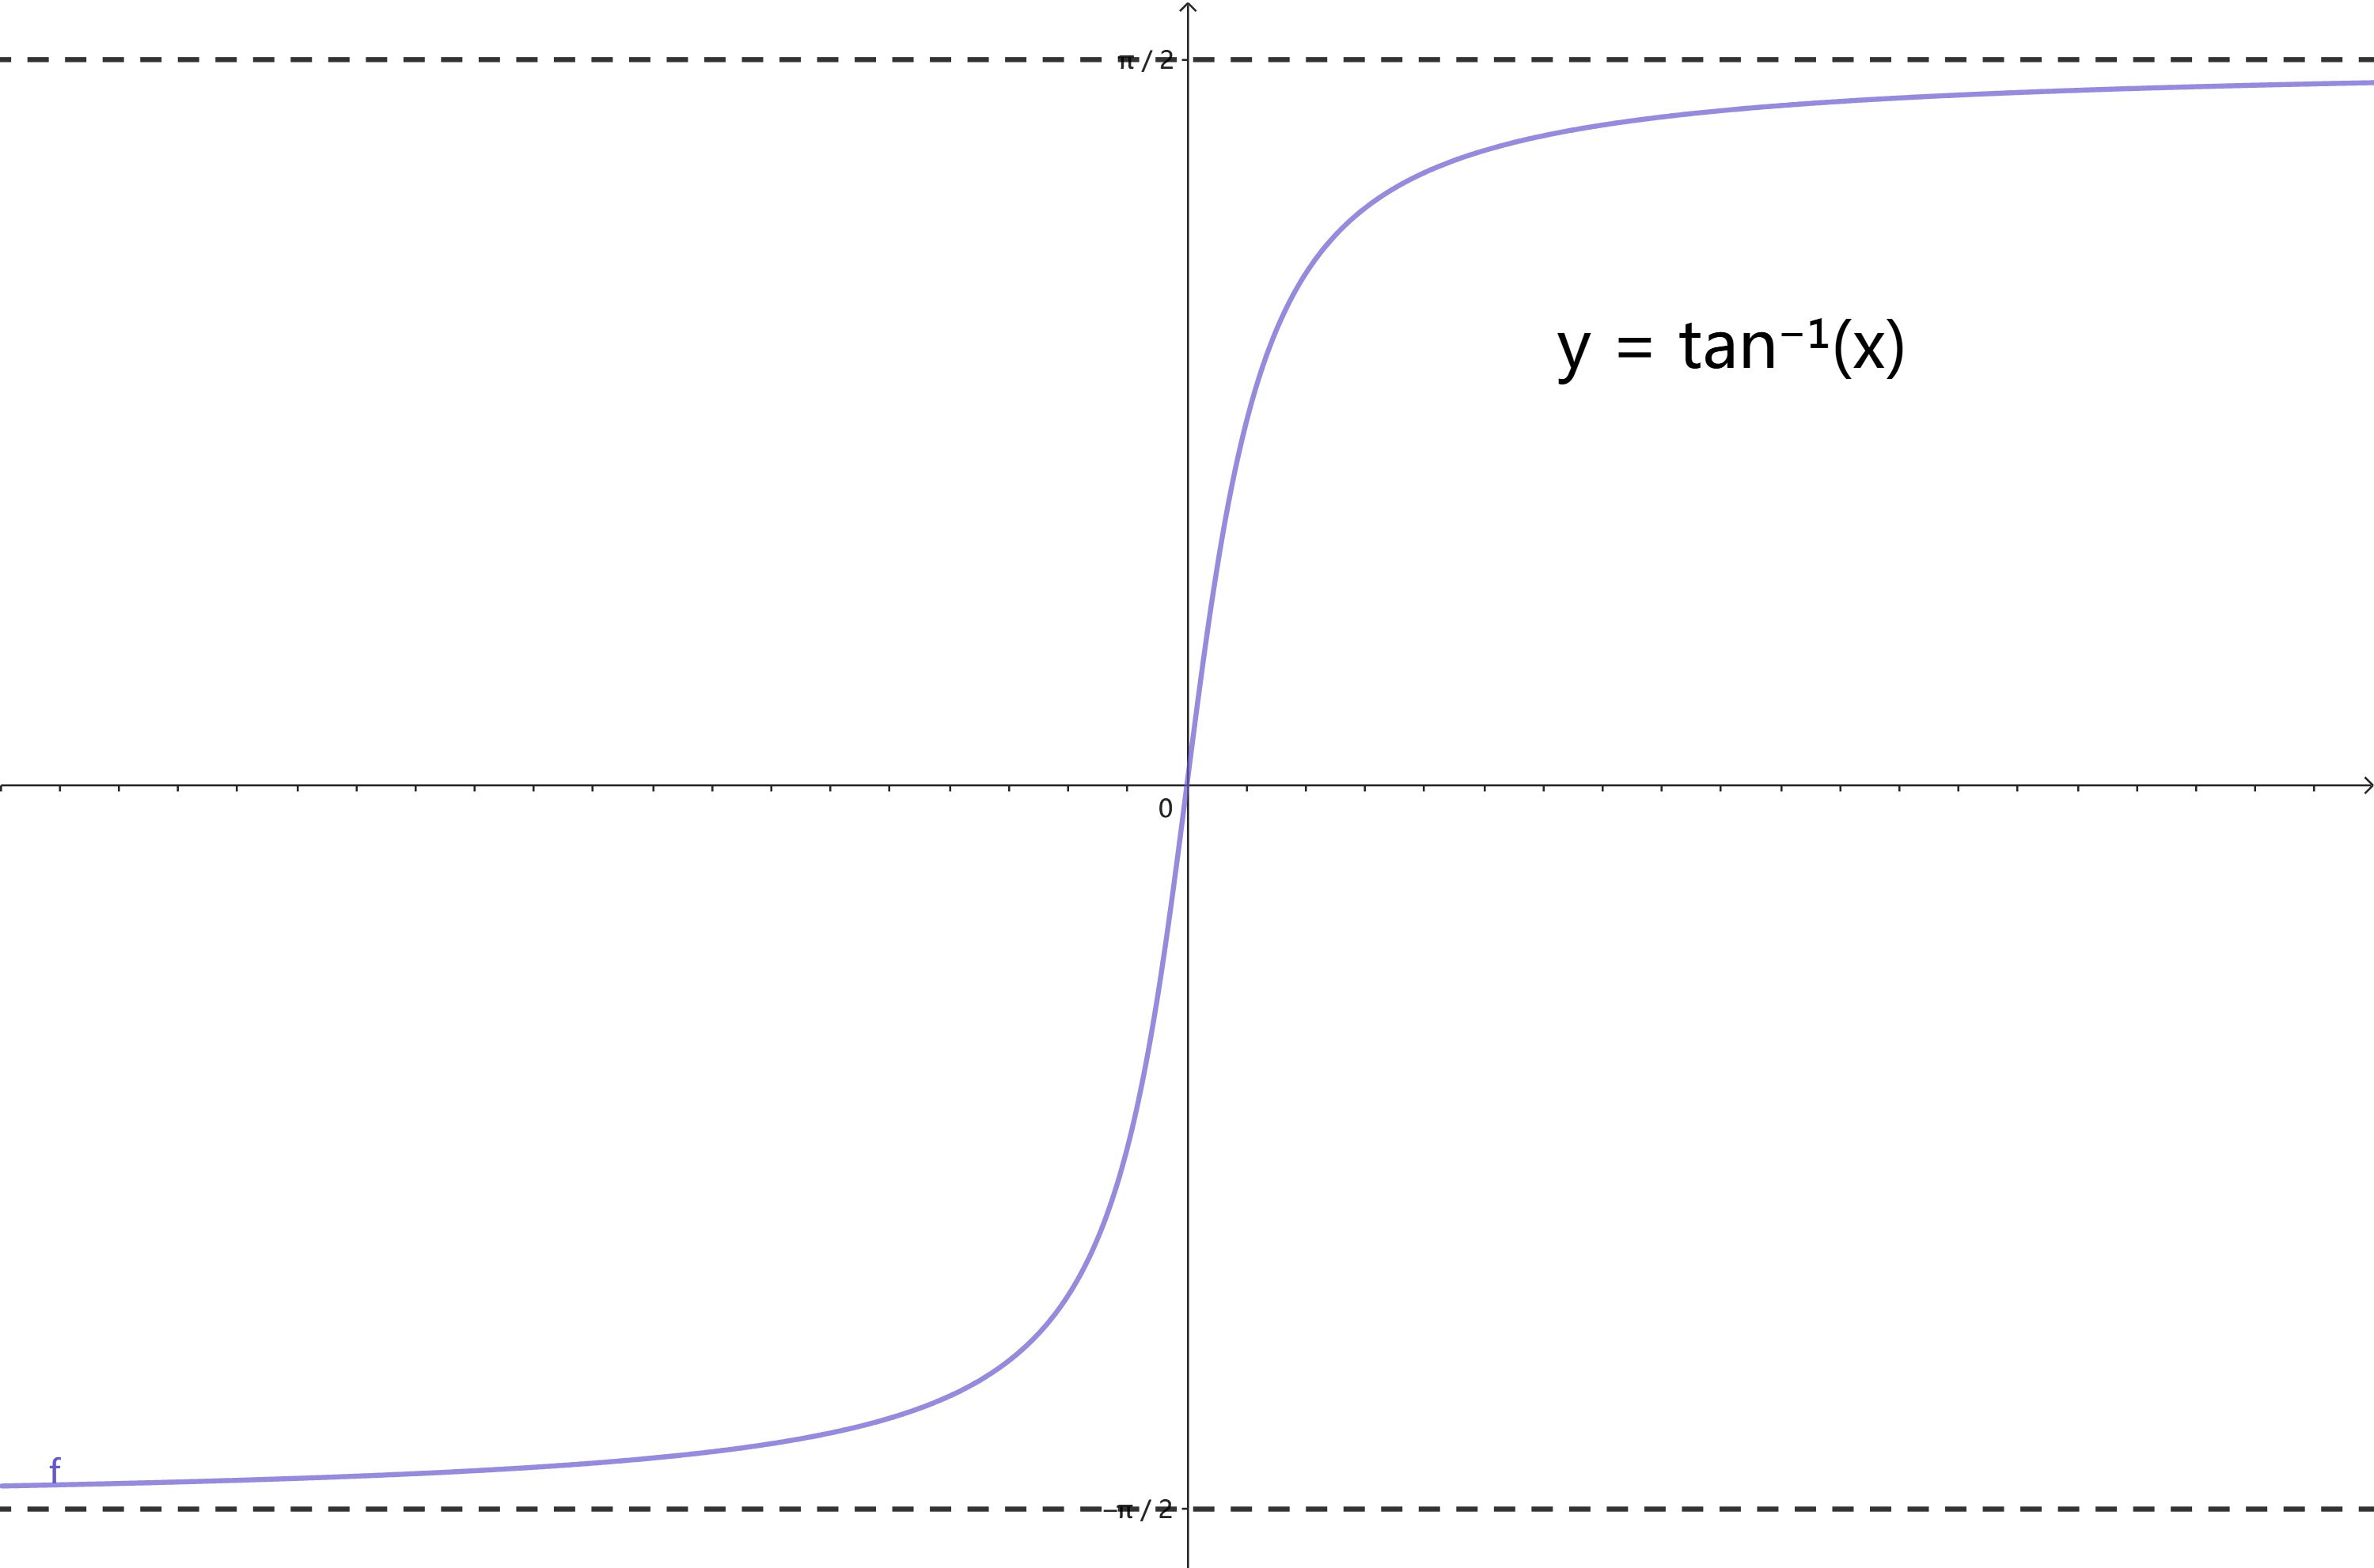
\includegraphics[width=\textwidth]{figure/arctan_plot.png}}
    \caption{} \label{arctan}
\end{minipage}
    \qquad
\begin{minipage}{0.4\linewidth}
    %\vspace{3pt}
    \centerline{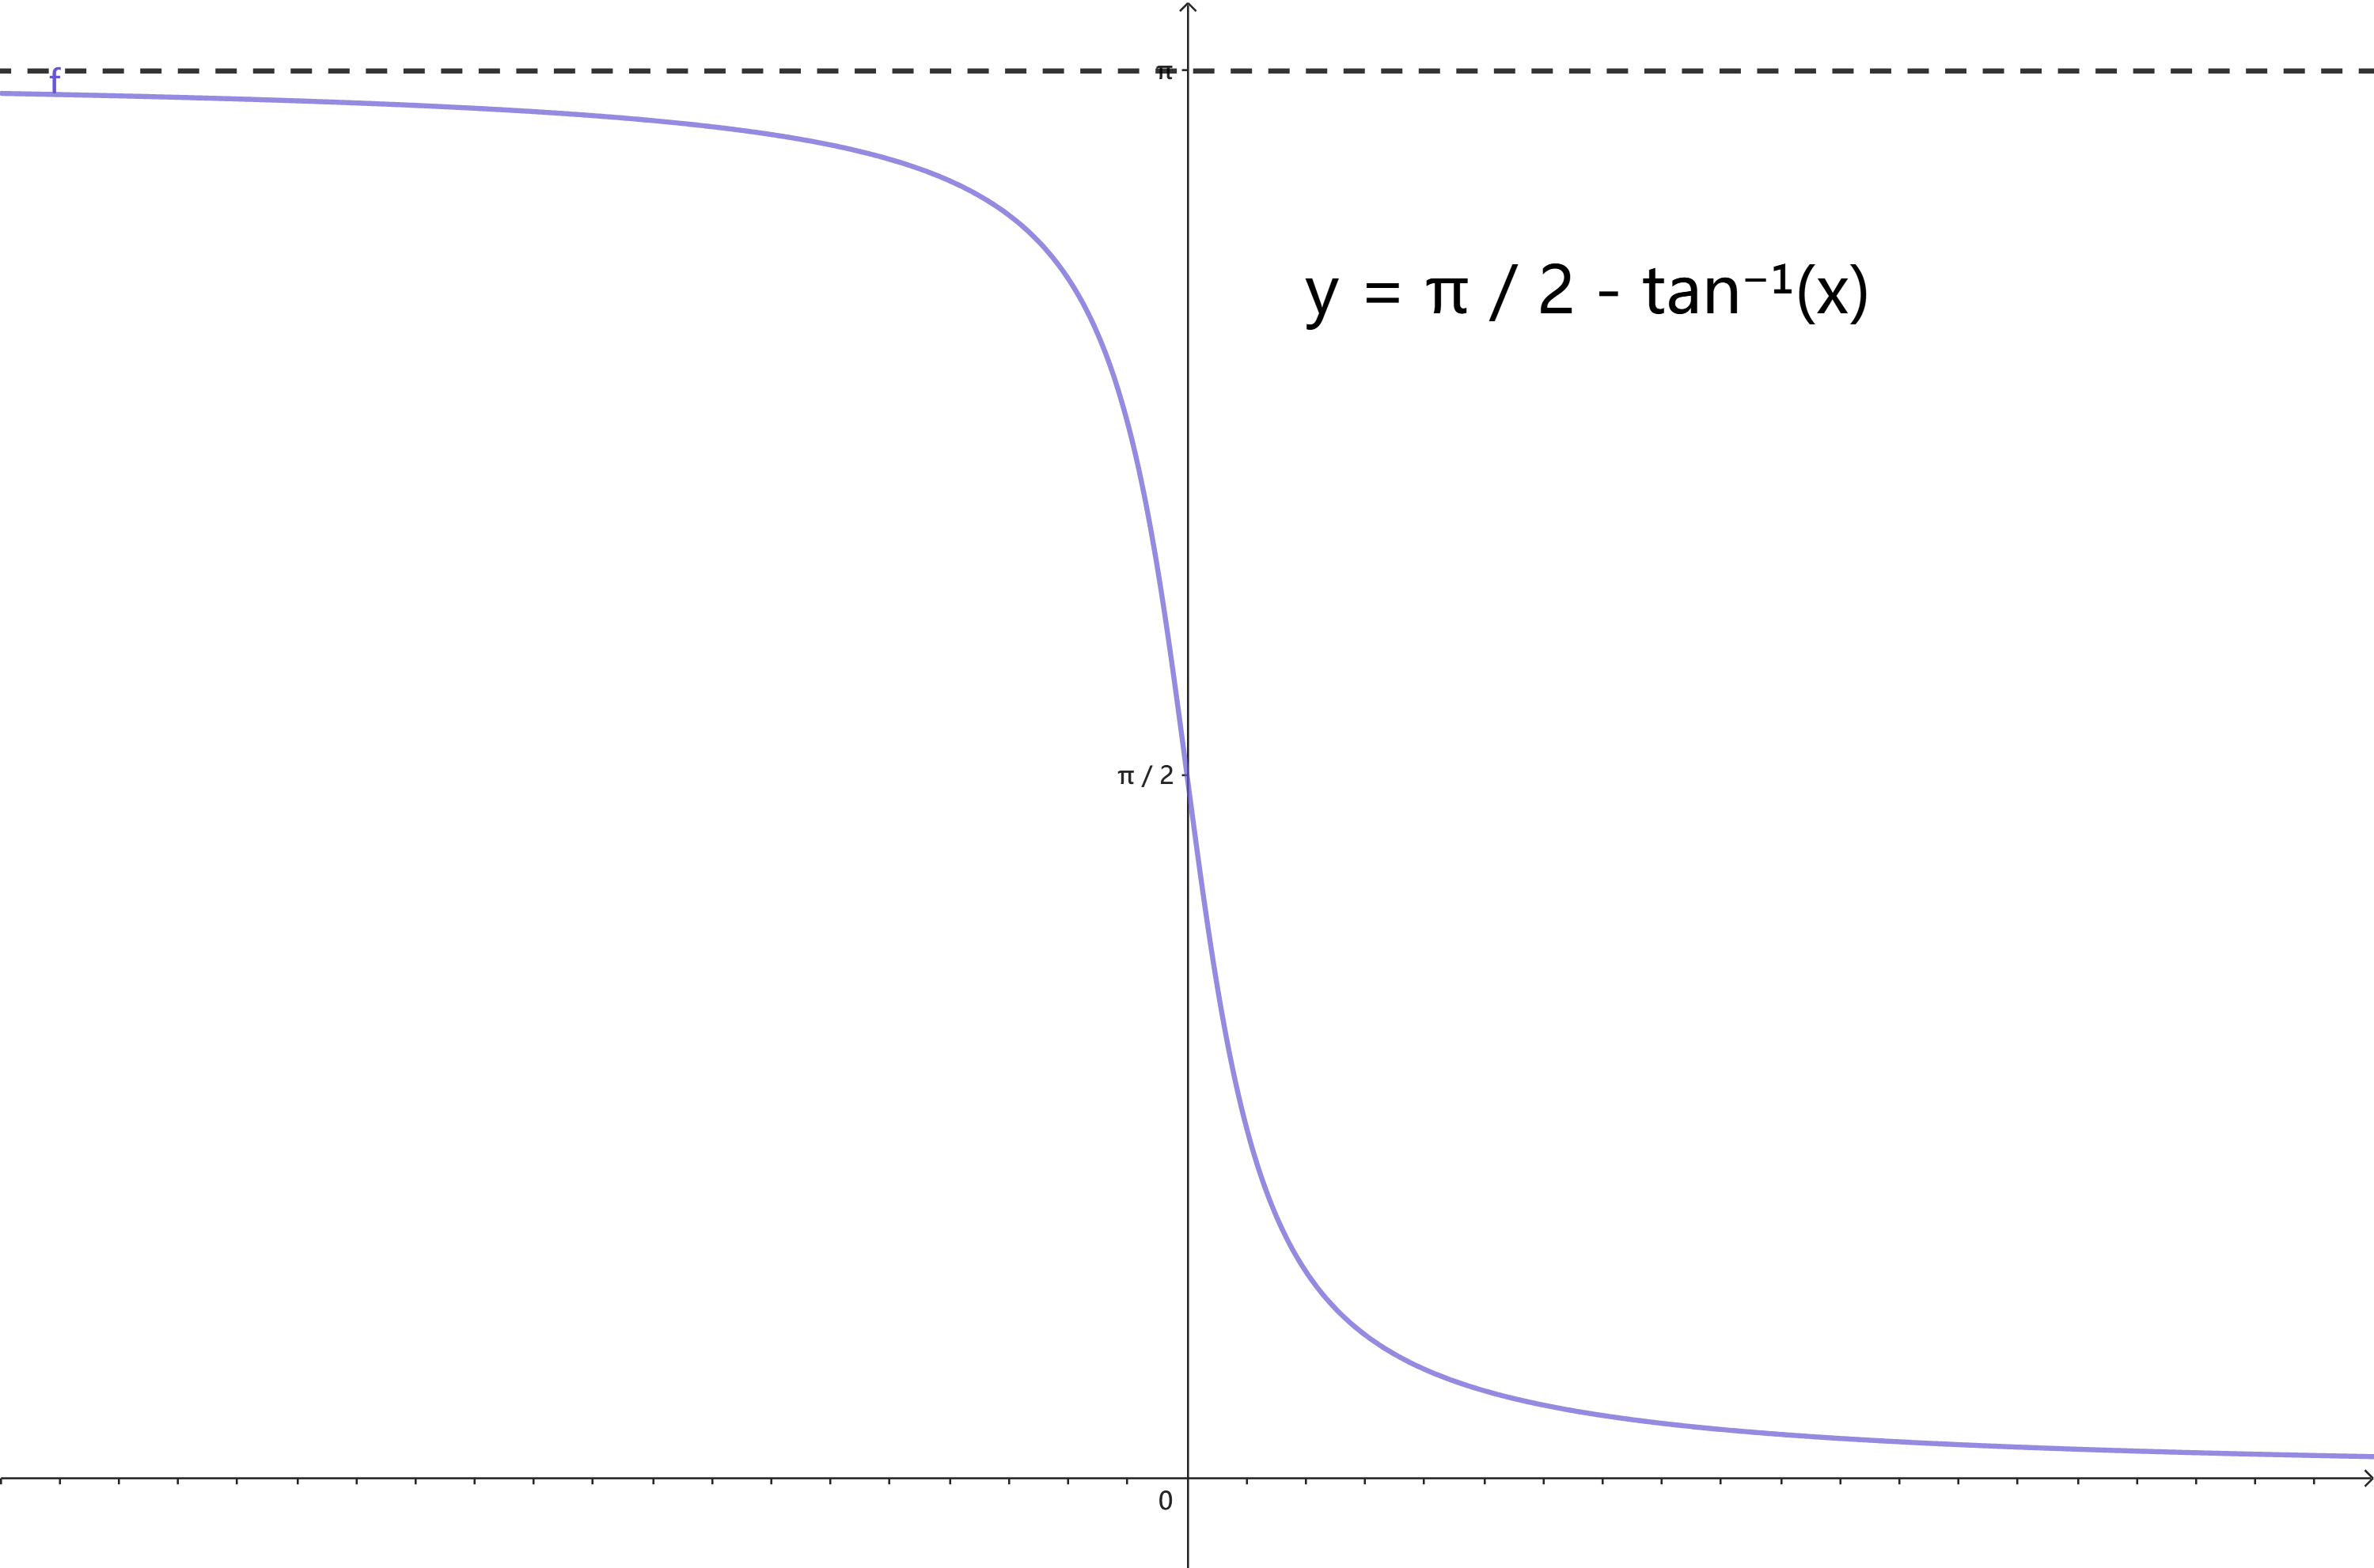
\includegraphics[width=\textwidth]{figure/arccot_plot.png}}
    \caption{} \label{arccot}
\end{minipage}
\end{figure}

$y=\arctan x$是$y=\tan x\left(-\dfrac{\pi}{2}< x< \dfrac{\pi}{2}\right)$的反函数,$y=\arccot x$是$y=\cot x(0< x< \pi)$的反函数

\begin{note}
    \begin{enumerate}
        \item 定义域:$(-\infty,+\infty)$

        值域:$y=\arctan x$的值域为$\left(-\dfrac{\pi}{2},\dfrac{\pi}{2}\right)$,$y=\arccot x$的值域为$(0,\pi)$。

        \item 单调性:$y=\arctan x$单调增加,$y=\arccot x$单调减少。

        \item 奇偶性:$y=\arctan x$为奇函数(在其定义域内)。

        \item 有界性:两个函数在其定义域内有界,$-\dfrac{\pi}{2}< \arctan x< \dfrac{\pi}{2}, 0< \arccot x<\pi$

        \item 性质:$\arctan x+\arccot x = \dfrac{\pi}{2}(-\infty< x <\infty)$
        \begin{proof}
            令$f(x)=\arctan x+\arccot x,-\infty< x <\infty$,则$f'(x)=\dfrac{1}{1+x^2}-\dfrac{1}{1+x^2}=0$,于是$f(x)=C$(常数),又$f(0)=\dfrac{\pi}{2}$,故$f(x)=\dfrac{\pi}{2}$,证毕。
        \end{proof}
        \vspace{2mm}

        \item 特殊函数值:
        \begin{equation}
        \begin{aligned}
            &
            \arctan 0 = 0, \quad \arctan \dfrac{\sqrt{3}}{3} = \dfrac{\pi}{6}, \quad \arctan 1 = \dfrac{\pi}{4}, \quad \arctan \sqrt{3} = \dfrac{\pi}{3} \\
            &
            \arccot 0 = \dfrac{\pi}{2}, \quad \arccot \sqrt{3} = \dfrac{\pi}{6}, \quad \arccot 1 = \dfrac{\pi}{4}, \quad \arccot \dfrac{\sqrt{3}}{3} = \dfrac{\pi}{3}
        \end{aligned}    \nonumber
        \end{equation}

        \item 极限:$\displaystyle \lim_{x\rightarrow -\infty} \arctan x = -\dfrac{\pi}{2}, \quad \lim_{x\rightarrow +\infty} \arctan x = \dfrac{\pi}{2}, \quad \lim_{x\rightarrow-\infty} \arccot x = \pi, \quad \lim_{x\rightarrow +\infty} \arccot x = 0$
    \end{enumerate}
\end{note}

\subsection{三角函数公式}
\textbf{三角函数基本关系}
\begin{equation}
    \begin{aligned}
        &\sin^2\alpha + \cos^2\alpha = 1 \\
        &1 + \tan^2\alpha = \sec^2\alpha \\
        &1 + \cot^2\alpha = \csc^2\alpha
    \end{aligned}\nonumber
\end{equation}

\textbf{倍角公式}
\begin{equation}
    \begin{aligned}
        & \sin 2\alpha = 2\sin\alpha\cos\alpha, \quad \cos 2\alpha = \cos^2\alpha-\sin^2\alpha = 1 - 2\sin^2\alpha = 2\cos^2\alpha - 1 \\
        & \sin 3\alpha = -4\sin^3\alpha+3\sin\alpha, \quad \cos 3\alpha = 4\cos^3\alpha-3\cos\alpha \\
        & \tan 2\alpha = \dfrac{2\tan\alpha}{1-\tan^2\alpha}, \quad \cot 2\alpha = \dfrac{\cot^2\alpha-1}{2\cot\alpha}
    \end{aligned}\nonumber
\end{equation}

\textbf{半角公式}
\begin{equation}
    \begin{aligned}
        & \sin^2\dfrac{\alpha}{2} = \dfrac{1}{2}(1-\cos\alpha), \quad \cos^2\dfrac{\alpha}{2} = \dfrac{1}{2}(1+\cos\alpha) \\
        & \sin\dfrac{\alpha}{2} = \pm\sqrt{\dfrac{1-\cos\alpha}{2}}, \quad \cos\dfrac{\alpha}{2} = \pm\sqrt{\dfrac{1+\cos\alpha}{2}} \\
        & \tan\dfrac{\alpha}{2} = \dfrac{1-\cos\alpha}{\sin\alpha}=\dfrac{\sin\alpha}{1+\cos\alpha}=\pm\sqrt{\dfrac{1-\cos\alpha}{1+\cos\alpha}} \\ 
        & \cot\dfrac{\alpha}{2} = \dfrac{\sin\alpha}{1-\cos\alpha} = \dfrac{1+\cos\alpha}{\sin\alpha} = \pm\sqrt{\dfrac{1+\cos\alpha}{1-\cos\alpha}}
    \end{aligned} \nonumber
\end{equation}

\textbf{和差公式}
\begin{equation}
    \begin{aligned}
        &\sin(\alpha\pm\beta)=\sin\alpha\cos\beta\pm\cos\alpha\sin\beta, \quad \cos(\alpha\pm\beta)=\cos\alpha\cos\beta\mp\sin\alpha\sin\beta \\
        &\tan(\alpha\pm\beta)=\dfrac{\tan\alpha\pm\tan\beta}{1\mp\tan\alpha\tan\beta}, \quad \cot(\alpha\pm\beta)=\dfrac{\cot\alpha\cot\beta\mp 1}{\cot\beta\pm\cot\alpha}
    \end{aligned}\nonumber
\end{equation}

\textbf{积化和差公式}
\begin{equation}
    \begin{aligned}
        &\sin\alpha\cos\beta = \dfrac{1}{2}[\sin(\alpha+\beta)+\sin(\alpha-\beta)], \quad \cos\alpha\sin\beta = \dfrac{1}{2}[\sin(\alpha+\beta)-\sin(\alpha-\beta)] \\
        &\cos\alpha\cos\beta = \dfrac{1}{2}[\cos(\alpha+\beta)+\cos(\alpha-\beta)], \quad \sin\alpha\sin\beta = \dfrac{1}{2} [\cos(\alpha-\beta)-\cos(\alpha+\beta)]
    \end{aligned} \nonumber
\end{equation}

\textbf{和差化积公式}
\begin{equation}
    \begin{aligned}
        &\sin\alpha+\sin\beta = 2\sin\dfrac{\alpha+\beta}{2}\cos\dfrac{\alpha-\beta}{2}, \quad \sin\alpha-\sin\beta=2\sin\dfrac{\alpha-\beta}{2}\cos\dfrac{\alpha+\beta}{2} \\
        &\cos\alpha+\cos\beta = 2\cos\dfrac{\alpha+\beta}{2}\cos\dfrac{\alpha-\beta}{2}, \quad \cos\alpha-\cos\beta=-2\sin\dfrac{\alpha+\beta}{2}\sin\dfrac{\alpha-\beta}{2}
    \end{aligned}\nonumber
\end{equation}

\textbf{万能公式}

若$u=\tan\dfrac{x}{2}(-\pi<x<\pi)$,则$\sin x=\dfrac{2u}{1+u^2}, \cos x=\dfrac{1-u^2}{1+u^2}$

\section{因式分解公式}
\begin{equation}
    \begin{aligned}
        &(a+b)^3=a^3+3a^2b+3ab^2+b^3, \quad (a-b)^3=a^3-3a^2b-3ab^2-b^3 \\
        &a^3-b^3=(a-b)(a^2+ab+b^2), \quad a^3+b^3=(a+b)(a^2-ab+b^2) \\
        &a^n-b^n=(a-b)(a^{n-1}+a^{n-2}b+\cdots+ab^{n-2}+b^{n-1})(n\mbox{是正整数}) \\
        &a^n-b^n=(a+b)(a^{n-1}-a^{n-2}b+\cdots-ab^{n-2}+b^{n-1})(n\mbox{为偶数}) \\
        &n\mbox{是正奇数时},a^n+b^n=(a+b)(a^{n-1}-a^{n-2}b+\cdots-ab^{n-2}+b^{n-1})
    \end{aligned} \nonumber \\
\end{equation}

\begin{equation}
    \begin{aligned}
        (a+b)^n=\sum_{k=0}^n\binom{n}{k}a^{n-k}b^k=
        &a^n+na^{n-1}b+\dfrac{n(n-1)}{2!}a^{n-2}b^2+\cdots+ \\
        &\dfrac{n(n-1)\cdots(n-k+1)}{k!}a^{n-k}b^k+\cdots+nab^{n-1}+b^n        
    \end{aligned}\nonumber
\end{equation}

\section{阶乘与双阶乘}
\begin{enumerate}
    \item $n!=1\cdot2\cdot3\cdot \ \cdots \ \cdot n$,规定$0!=1$。
    \item $(2n)!!=2\cdot4\cdot6\cdot \ \cdots \cdot (2n)=2^n\cdot n!$
    \item $(2n-1)!!=1\cdot3\cdot5\cdot \ \cdots \ \cdot (2n-1)$
\end{enumerate}

\section{常用不等式}
\begin{enumerate}
    \item 设$a,b$为实数,则(1)$\left|a\pm b\right|\leq\left|a\right|+\left|b\right|$;(2)$\left|\left|a\right|-\left|b\right|\right|\leq\left|a-b\right|$
    
    \item (1)$\sqrt{ab}\leq\dfrac{a+b}{2}\leq\sqrt{\dfrac{a^2+b^2}{2}} \quad (a,b>0)$ \\
    (2)$\sqrt[3]{abc}\leq\dfrac{a+b+c}{3}\leq\sqrt{\dfrac{a^2+b^2+c^3}{3}} \quad (a,b,c>0)$

    \item 若$0<a<x<b,0<c<y<d$,则$\dfrac{c}{b}<\dfrac{y}{x}<\dfrac{d}{a}$

    \item $\sin x<x< \tan x \quad \left( 0<x<\dfrac{\pi}{2} \right)$

    \item $\sin x<x \quad (x>0)$

    \item $\arctan x\leq x\leq \arcsin x \quad (0\leq x\leq 1)$

    \item $e^x\geq x+1 \quad (\forall x)$

    \item $x-1\geq\ln x \quad (x>0)$

    \item $\dfrac{1}{x+1}<\ln(1+\dfrac{1}{x})<\dfrac{1}{x} \quad (x>0)$
\end{enumerate}
